%%%%%%%%%%%%%%%%%%%%%%%%%%%%%%%%%%%%%
\section{Methods}
\label{sec:Methods}

For convince a subversion repository was created to manage the developed code base, and all source code is available by anonymous checkout from \verb+http://www.murphs-code-repository.googlecode.com/svn/trunk/layeredPolymerTracking+. Revision 360 was the code base used to generate the results shown in \ref{sec:Results}.

\subsubsection{Detector Geometry}
A detector geometry in GEANT4 is made up of a number of volumes.
The largest volume is the \verb+world+ volume which contains all other volumes in the detector geometry.
Each volume (an instance of \verb+G4VPhysicalVolume+) by assining a position, a pointer to the mother volume and a pointer to its mother volume (or \verb+NULL+ if it is the \verb+world+ volume).
A volume's shape is described by \verb+G4VSolid+ which has a shpae and the specific values for each dimension.
A volume's full properties is described by a logical volume.
A \verb+G4LogicalVolume+ includes a pointer to the geometrical properties of the volume (the solid) along with physcial charactersics including:
\begin{itemize}
    \item the material of the volume,
    \item sensitive detectors of the volume and,
    \item any magnetic fields.
\end{itemzie}
Listing \ref{lst:World} provides the implemenation of the world physical volume.
The geometry was setup such that it is possible to define multiple layers of detectors, as shown in Figure \ref{fig:LayerDetectorGeo}.
%%%%%%%%%%%%%%%%%%%%%%%%% LISTING CODE %%%%%%%%%%%%%%%%%%%%%%%%%%
\begin{lstlisting}[style=MyCStyle,caption=World Physical Volume,label=lst:World]
    // World
    worldS = new G4Box("World",worldSizeXY, worldSizeXY, worldSizeZ*0.5); 
    worldLV = new G4LogicalVolume(worldS,defaultMaterial,"World");
    worldPV = new G4PVPlacement(0,G4ThreeVector(),worldLV,"World",0,false,0,fCheckOverlaps);

\end{lstlisting}
%%%%%%%%%%%%%%%%%%%%%%%%% LISTING CODE %%%%%%%%%%%%%%%%%%%%%%%%%%
\begin{lstlisting}[style=MyCStyle,caption=Listing,label=lst:label]

\end{lstlisting}

\begin{figure} 
    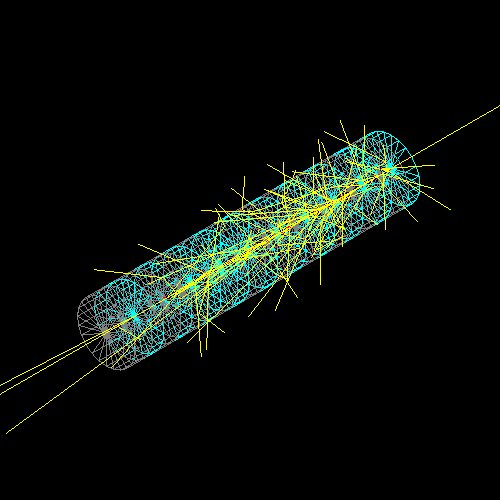
\includegraphics[width=\figurewidth]{10LayerGamma}
	\caption{10 Layer Detector with a simulated gamma event}
    \label{fig:LayerDetectorGeo}
\end{figure}
\subsubsection{Physics Lists}
